\documentclass[border=4pt]{standalone}

\usepackage{amsmath}
\usepackage{tikz}
\usepackage{mathdots}
\usepackage{yhmath}
\usepackage{cancel}
\usepackage{color}
\usepackage{siunitx}
\usepackage{array}
\usepackage{multirow}
\usepackage{amssymb}
\usepackage{gensymb}
\usepackage{tabularx}
\usepackage{booktabs}
\usetikzlibrary{fadings}
\usetikzlibrary{patterns}


\begin{document}
 


\tikzset{every picture/.style={line width=0.75pt}} %set default line width to 0.75pt        

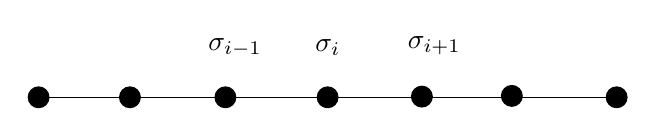
\begin{tikzpicture}[x=0.75pt,y=0.75pt,yscale=-1,xscale=1]
%uncomment if require: \path (0,300); %set diagram left start at 0, and has height of 300

%Straight Lines [id:da27990377163976854] 
\draw    (100,116) -- (378.5,116) ;


%Shape: Circle [id:dp2612476085751765] 
\draw  [fill={rgb, 255:red, 0; green, 0; blue, 0 }  ,fill opacity=1 ] (95,116) .. controls (95,113.24) and (97.24,111) .. (100,111) .. controls (102.76,111) and (105,113.24) .. (105,116) .. controls (105,118.76) and (102.76,121) .. (100,121) .. controls (97.24,121) and (95,118.76) .. (95,116) -- cycle ;
%Shape: Circle [id:dp6080793711393817] 
\draw  [fill={rgb, 255:red, 0; green, 0; blue, 0 }  ,fill opacity=1 ] (373.5,116) .. controls (373.5,113.24) and (375.74,111) .. (378.5,111) .. controls (381.26,111) and (383.5,113.24) .. (383.5,116) .. controls (383.5,118.76) and (381.26,121) .. (378.5,121) .. controls (375.74,121) and (373.5,118.76) .. (373.5,116) -- cycle ;
%Shape: Circle [id:dp6980421772102914] 
\draw  [fill={rgb, 255:red, 0; green, 0; blue, 0 }  ,fill opacity=1 ] (323,115.33) .. controls (323,112.57) and (325.24,110.33) .. (328,110.33) .. controls (330.76,110.33) and (333,112.57) .. (333,115.33) .. controls (333,118.09) and (330.76,120.33) .. (328,120.33) .. controls (325.24,120.33) and (323,118.09) .. (323,115.33) -- cycle ;
%Shape: Circle [id:dp04398531477348322] 
\draw  [fill={rgb, 255:red, 0; green, 0; blue, 0 }  ,fill opacity=1 ] (139,116) .. controls (139,113.24) and (141.24,111) .. (144,111) .. controls (146.76,111) and (149,113.24) .. (149,116) .. controls (149,118.76) and (146.76,121) .. (144,121) .. controls (141.24,121) and (139,118.76) .. (139,116) -- cycle ;
%Shape: Circle [id:dp09808275234723718] 
\draw  [fill={rgb, 255:red, 0; green, 0; blue, 0 }  ,fill opacity=1 ] (234.25,116) .. controls (234.25,113.24) and (236.49,111) .. (239.25,111) .. controls (242.01,111) and (244.25,113.24) .. (244.25,116) .. controls (244.25,118.76) and (242.01,121) .. (239.25,121) .. controls (236.49,121) and (234.25,118.76) .. (234.25,116) -- cycle ;
%Shape: Circle [id:dp6441912130696283] 
\draw  [fill={rgb, 255:red, 0; green, 0; blue, 0 }  ,fill opacity=1 ] (279.67,115.67) .. controls (279.67,112.91) and (281.91,110.67) .. (284.67,110.67) .. controls (287.43,110.67) and (289.67,112.91) .. (289.67,115.67) .. controls (289.67,118.43) and (287.43,120.67) .. (284.67,120.67) .. controls (281.91,120.67) and (279.67,118.43) .. (279.67,115.67) -- cycle ;
%Shape: Circle [id:dp2668399358209168] 
\draw  [fill={rgb, 255:red, 0; green, 0; blue, 0 }  ,fill opacity=1 ] (185,116) .. controls (185,113.24) and (187.24,111) .. (190,111) .. controls (192.76,111) and (195,113.24) .. (195,116) .. controls (195,118.76) and (192.76,121) .. (190,121) .. controls (187.24,121) and (185,118.76) .. (185,116) -- cycle ;

% Text Node
\draw (194.67,92) node    {$\sigma _{i-1}$};
% Text Node
\draw (290.67,91.33) node    {$\sigma _{i+1}$};
% Text Node
\draw (239.33,92) node    {$\sigma _{i}$};


\end{tikzpicture}



\end{document}
